\subsection{Configuración del Almacenamiento en Bacula}

Primero, creamos un directorio para almacenar los respaldos y asignamos los permisos adecuados para que Bacula pueda gestionar los archivos.

\begin{figure}[H]
    \centering
    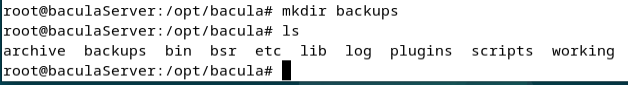
\includegraphics[width=0.5\linewidth]{instalacionBacula/mkdirbackups.png}
    \caption{Creación del directorio de respaldos en el servidor Bacula}
\end{figure}

En Webmin, navegamos a la configuración de dispositivos de almacenamiento de Bacula para agregar un nuevo dispositivo que apunte al directorio que acabamos de crear.

\begin{figure}[H]
    \centering
    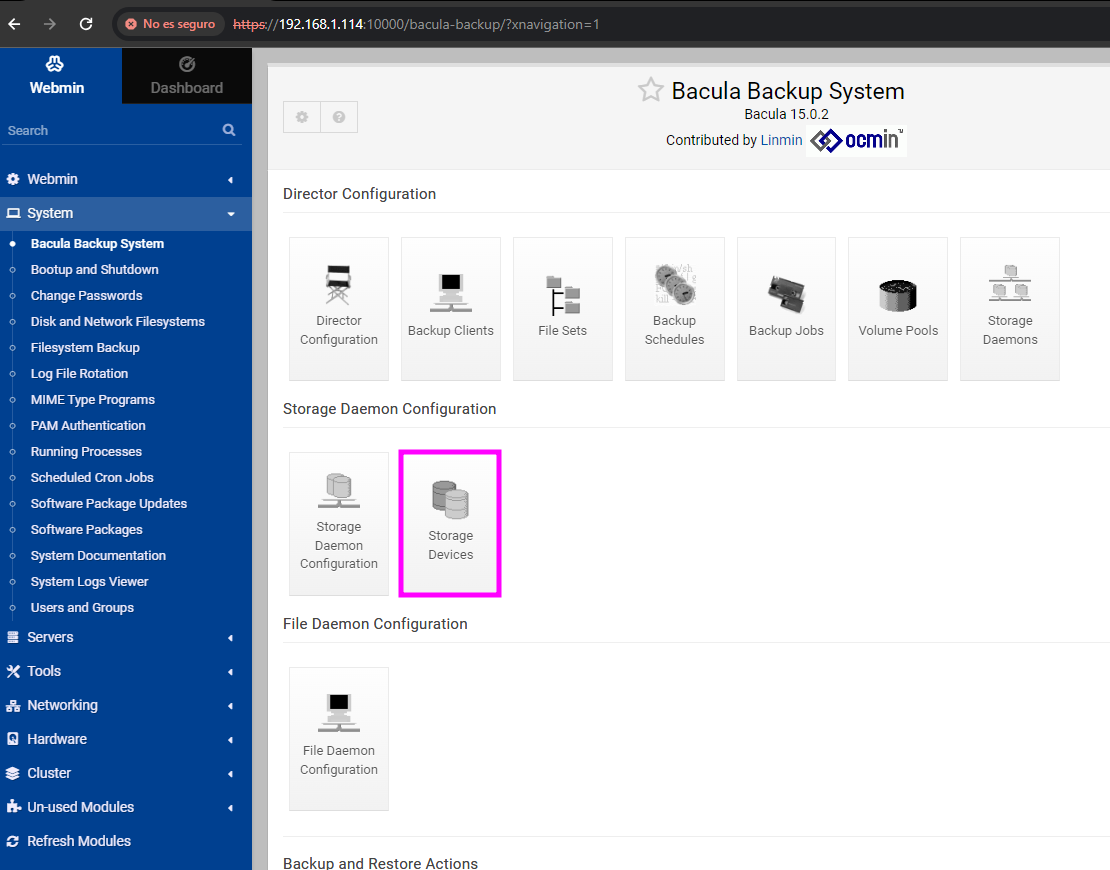
\includegraphics[width=0.5\linewidth]{instalacionBacula/STO.png}
    \caption{Interfaz de configuración de dispositivos de almacenamiento en Webmin}
\end{figure}

Agregamos un nuevo dispositivo de almacenamiento local en Webmin con los siguientes detalles \textbf{Nombre del dispositivo de almacenamiento:} localBackups; \textbf{Directorio o archivo del dispositivo:} /opt/bacula/backups; \textbf{Nombre del tipo de medio:} localBackups.



\begin{minipage}[t]{0.45\textwidth}
    \vspace{0pt} % Alinea la parte superior de la minipágina con lo que esté al lado
    \begin{figure}[H]
        \centering
        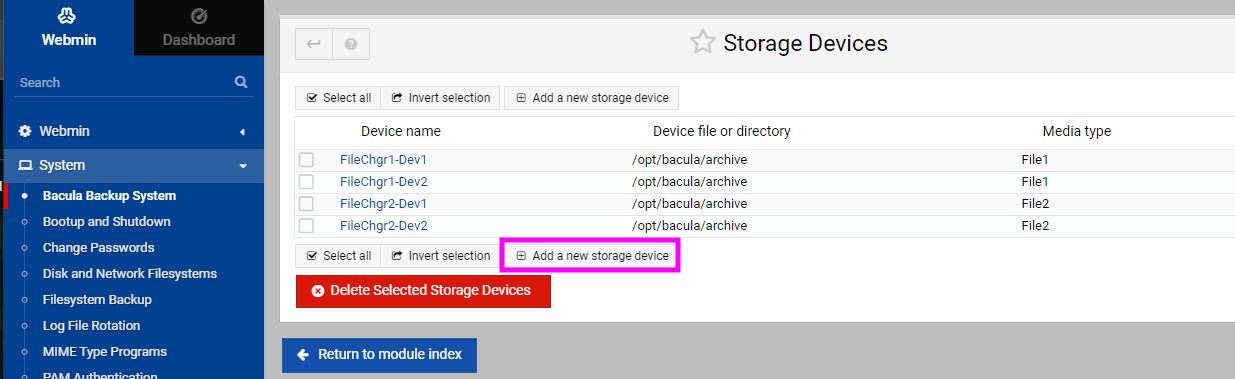
\includegraphics[width=0.95\linewidth]{instalacionBacula/NSD.png}
        \caption{Creación de un nuevo dispositivo de almacenamiento en Webmin}
    \end{figure}    
    \end{minipage}%
    \hfill % Añade espacio entre las dos minipáginas si es necesario
    \begin{minipage}[t]{0.45\textwidth}
    \vspace{0pt} % Alinea la parte superior de la minipágina con lo que esté al lado
    \centering % Centra el contenido de la minipágina
        \begin{figure}[H]
            \centering
            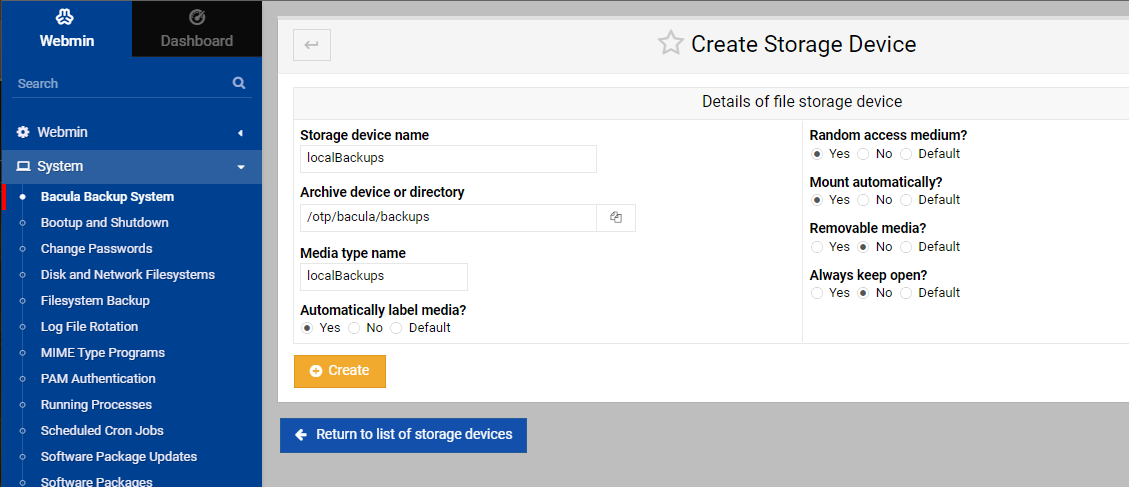
\includegraphics[width=0.95\linewidth]{instalacionBacula/localbac.png}
            \caption{Detalles del nuevo dispositivo de almacenamiento creado en Webmin}
        \end{figure}
    \end{minipage}
    
\medskip



%añadir opciones


Procedemos a configurar el daemon de almacenamiento para manejar las solicitudes de almacenamiento de datos.

\begin{figure}[H]
    \centering
    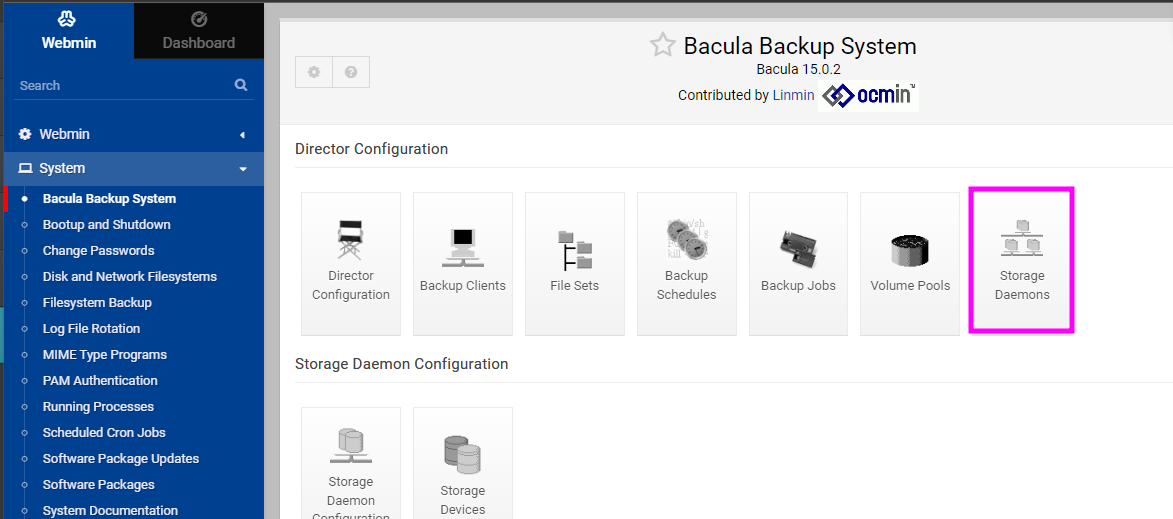
\includegraphics[width=0.5\linewidth]{instalacionBacula/stdeamon.png}
    \caption{Configuración inicial del daemon de almacenamiento en Webmin}
\end{figure}

Añadimos un nuevo daemon de almacenamiento especificando la IP del servidor y el puerto que Bacula utilizará para la comunicación. Esto facilita la gestión y evita la necesidad de configurar nombres de host o DNS en entornos sin estas facilidades.

\begin{figure}[H]
    \centering
    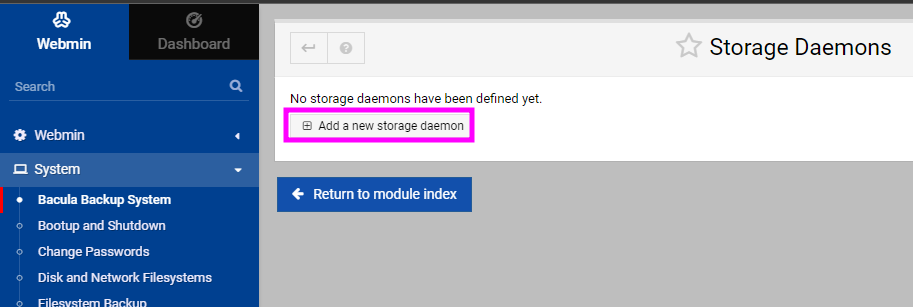
\includegraphics[width=0.5\linewidth]{instalacionBacula/newsd.png}
    \caption{Añadiendo un nuevo daemon de almacenamiento en Webmin}
\end{figure}

Finalmente, configuramos y creamos un pool de volúmenes donde Bacula almacenará los backups. Especificamos el nombre del pool, el tipo de pool, y configuramos opciones como el periodo de retención y la capacidad máxima de los volúmenes.



\begin{minipage}[t]{0.45\textwidth}
    \vspace{0pt} % Alinea la parte superior de la minipágina con lo que esté al lado
    \begin{figure}[H]
        \centering
        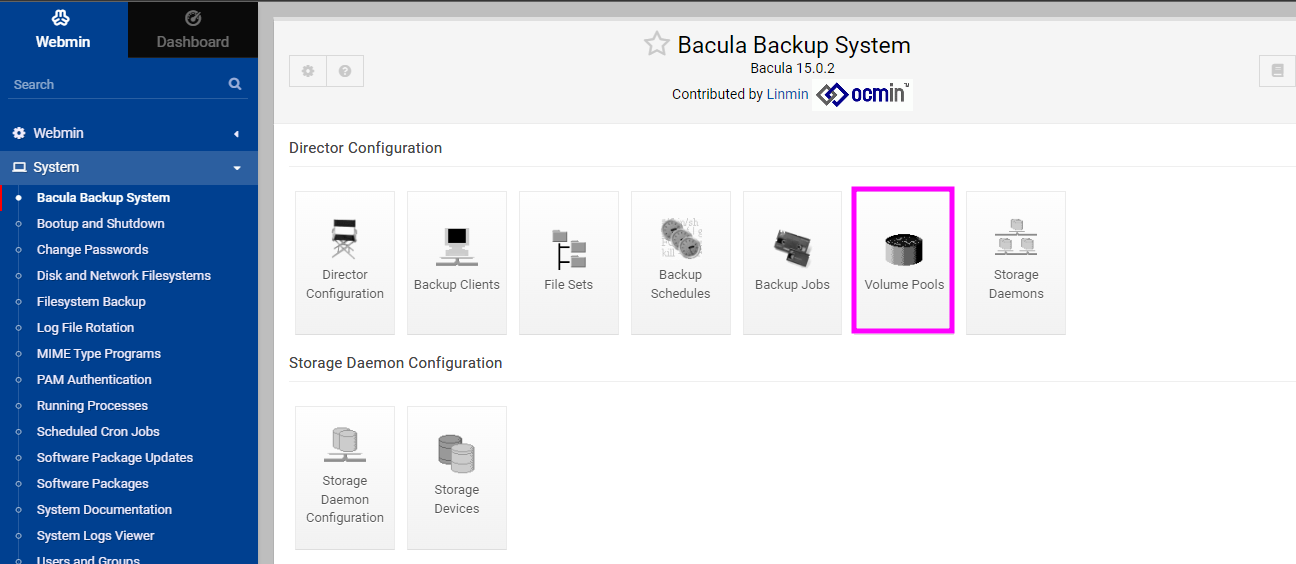
\includegraphics[width=0.95\linewidth]{instalacionBacula/pollv.png}
        \caption{Pool de volúmenes en Webmin}
    \end{figure} 
    \end{minipage}%
    \hfill % Añade espacio entre las dos minipáginas si es necesario
    \begin{minipage}[t]{0.45\textwidth}
    \vspace{0pt} % Alinea la parte superior de la minipágina con lo que esté al lado
    \centering % Centra el contenido de la minipágina
    \begin{figure}[H]
        \centering
        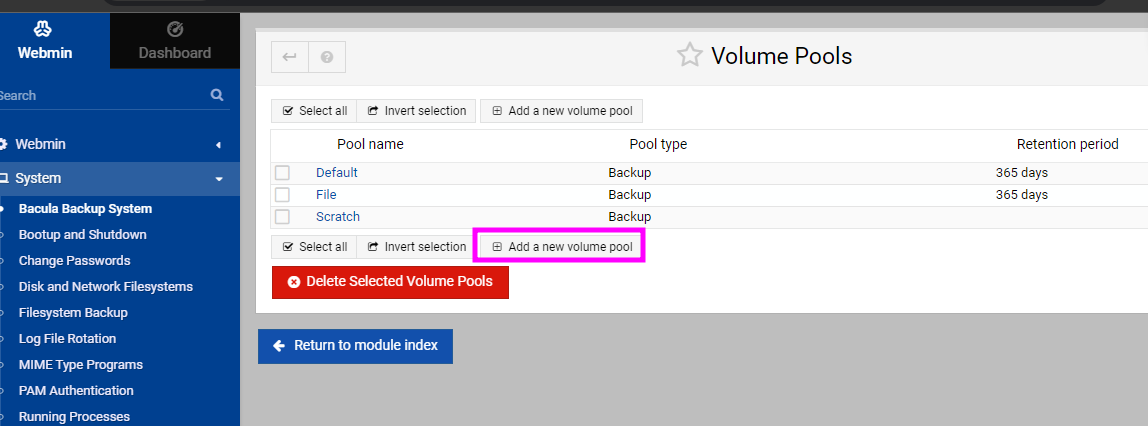
\includegraphics[width=0.95\linewidth]{instalacionBacula/pool22.png}
        \caption{Creación de un nuevo pool de volúmenes en Webmin}
    \end{figure}
    \end{minipage}
    
\medskip






Ahora para  configurar el volumen:
\begin{figure}[H]
    \centering
    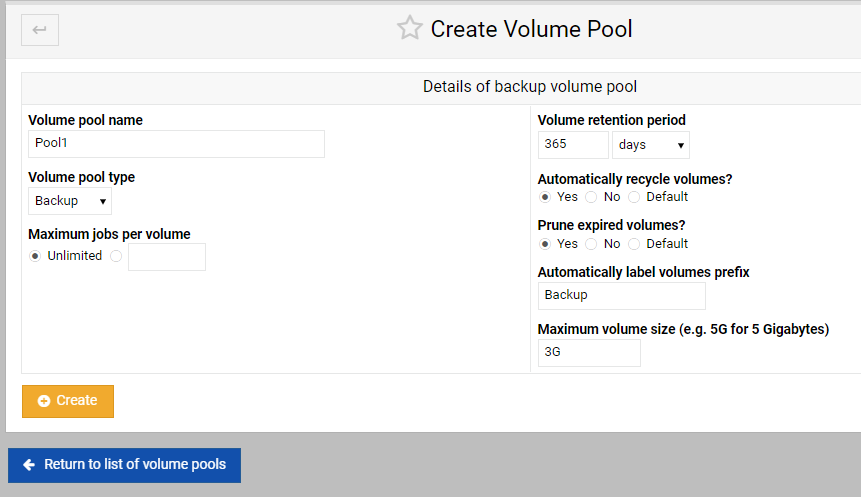
\includegraphics[width=0.5\linewidth]{instalacionBacula/createVolumePool.png}
    \caption{Configuración de detalles del pool de volúmenes en Webmin}
\end{figure}